\documentclass{article}


% if you need to pass options to natbib, use, e.g.:
%     \PassOptionsToPackage{numbers, compress}{natbib}
% before loading neurips_2024

% submissions should not be anonymous, so use the 
% [preprint] option:
\usepackage[preprint]{paper}


% to avoid loading the natbib package, add option nonatbib:
%    \usepackage[nonatbib,preprint]{neurips_2024}


\usepackage[utf8]{inputenc} % allow utf-8 input
\usepackage[T1]{fontenc}    % use 8-bit T1 fonts
\usepackage{hyperref}       % hyperlinks
\usepackage{url}            % simple URL typesetting
\usepackage{booktabs}       % professional-quality tables
\usepackage{amsfonts}       % blackboard math symbols
\usepackage{nicefrac}       % compact symbols for 1/2, etc.
\usepackage{microtype}      % microtypography
\usepackage{xcolor}         % colors
\usepackage{geometry}
\usepackage{longtable}
\usepackage{graphicx}
\usepackage{amsmath}
\usepackage{booktabs}
\usepackage{caption}

\title{Smart Model Elimination for Efficient Automated Machine Learning in Healthcare}


% The \author macro works with any number of authors. There are two commands
% used to separate the names and addresses of multiple authors: \And and \AND.
%
% Using \And between authors leaves it to LaTeX to determine where to break the
% lines. Using \AND forces a line break at that point. So, if LaTeX puts 3 of 4
% authors names on the first line, and the last on the second line, try using
% \AND instead of \And before the third author name.


\author{%
  Eric Su Zhang$^1$ \\
  St. Mark's School of Texas\\
  10600 Preston Rd, Dallas, TX 75230\\
  \texttt{26zhange@smtexas.org} \\
  % examples of more authors
  \And
  Benjamin Joseph Michael Standefer$^2$ \\
  St. Mark's School of Texas \\
  10600 Preston Rd, Dallas, TX 75230 \\
  \texttt{26standeferb@smtexas.org} \\
  % \AND
  % Coauthor \\
  % Affiliation \\
  % Address \\
  % \texttt{email} \\
  % \And
  % Coauthor \\
  % Affiliation \\
  % Address \\
  % \texttt{email} \\
  % \And
  % Coauthor \\
  % Affiliation \\
  % Address \\
  % \texttt{email} \\
}


\begin{document}


\maketitle


\begin{abstract}
  Automated Machine Learning (AutoML) has emerged as a popular field of research. We present a literature review of existing AutoML papers and conduct a survey on five popular AutoML frameworks. Typically, these frameworks engage in model selection by requiring every model to be run and assessed, a process both time-intensive and computationally expensive. In response, we propose a novel framework, Smart Model Elimination Machine Learning (SMEML), that strategically eliminates models that are unlikely to yield high accuracy. SMEML demonstrates the ability to achieve comparable accuracy to a traditional brute-force approach while significantly reducing the time required. We also believe this innovation is particularly beneficial to machine learning in healthcare, where efficient and accurate disease prediction is crucial. 
\end{abstract}


\section{Introduction}

Machine learning (ML) algorithms require complicated processes like hyperparamater tuning, and can be modified in conjunction with one another, like in ensemble learning. To do this on a larger scale and at greater speeds, recent research and effort have been put into developing AutoML frameworks. These frameworks create comfortable environments in which models can excel. They handle missing values, preprocess data, and optimize training to ensure the best results [1].

One sector of the global industry that has the most potential for beneficial integration of AutoML frameworks is healthcare, particularly in developing countries. These countries have severe shortages of healthcare workers and limited tools for diagnosis. For example, Africa has 2.3 healthcare workers per 1000 individuals, while the Americas have 24.8 healthcare workers per 1000 [2]. The World Health Organization (WHO) emphasized that this deficit is growing every year and will likely reach 18 million personnel by 2030 [3]. Medical AIs typically automate repetitive tasks, making time consumption a primary concern [4]. This coupled with a lack of adequate resources makes designing faster diagnostic systems for developing countries' medical sectors a pivotal issue. 

Most AutoML frameworks implement some form of model selection where a pool of models are filtered until a final model is selected. However, these frameworks require that every model be run [1]. In theory, this means that much energy is spent training models that are unlikely to be selected. We propose SMEML, a novel model selection algorithm that automatically eliminates models that it believes will not be performant. 

\subsection{Survey}

\begin{table}
  \caption{Survey of Existing AutoML Frameworks}
  \label{automl-survey}
  \centering
  \begin{tabular}{lllllllll}
    \toprule
    Framework & EOU & M & FE & TM & HPT & Inter & Custom\\
    \midrule
    H2O AutoML [5] & Easy & 12 & Basic & Yes & Auto & SHAP & High\\
    TPOT [6] & Hard & 10 & Basic & No & Genetic & POJO & Moderate\\
    MLJAR [7,8] & Easy & 12 & Advanced & Yes & Auto & Basic & High\\
    FLAML [9] & Easy & 9 & Limited & Yes & Auto & SHAP & Low-Moderate\\
    LightAutoML [10] & Easy & 11 & Advanced & Yes & Auto & Basic & Moderate\\
    \bottomrule
  \end{tabular}
  \captionsetup{font=footnotesize}
  \caption*{\textbf{Abbreviations}: EOU: Ease of Use, M: \# of models evaluated by framework, FE: Feature Engineering, TM: Time Management, HPT: Hyper-Parameter Tuning, Inter: Interface, Custom: Customization}
\end{table}
We systematically review and compare five different AutoML frameworks, comparing every feature relevant to medical implementation in Table 1. Of these five, we wanted to take a closer look at four: FLAML, H2O, MLJAR, and TPOT.

We can observe pros and cons in the four models' theoretical applications. FLAML uses blend search hyper-parameter optimization and focuses on lightweight models, making it quick and applicable to repetitive tasks. It supports user-specified imputation techniques for missing values and has an intuitive API, making it moderately user-friendly for healthcare workers [9]. H2O has a wider variety of supported algorithms that may be appropriate for medical diagnosis, making it slower than FLAML on average. In one trial, more than half of FLAML's performances in one minute were better than or equal to H2O's performances in one hour [9]. H2O has automatic and multi-faceted methods of dealing with missing values and flexible interfaces in R and Python, making it intuitive for users [5]. MLJAR uses advanced algorithms such as light gradient boosting and neural networks. It automatically deals with missing values and is known for its automated user interface [7]. TPOT uses genetic programming. It builds pipelines over multiple generations, which can be time consuming. It has built-in pre-processing for missing values, but the genetic programming requires fine-tuning from users [6].

Through this survey, we uncovered a key continuity in these frameworks' design: frameworks must run all of their models to maximize accuracy at the expense of efficiency. Given the specific nature of certain tabular data, there are some models that are less likely to perform well, thus running and training these models is wasteful. Cutting these models completely, however, is not optimal, as they are the best option in a minority of cases. We hypothesized that using a combination of multi-layer machine learning implementation and meta-feature extraction would yield an equally versatile system that minimizes time spent on training without sacrificing accuracy.

\section{Methodology}
When considering a specific dataset, the distribution, relationship between datapoints, and various other attributes can give us clues as to which models are likely to perform best. For example, linear models tend to work better on datasets where there is a linear relationship between features [11]. Accordingly, we can develop a boosting model to predict the best models based on extracted attributes from a dataset. These extracted attributes are shown in Table 2. Each attribute attempts to capture a specific type of relationship or distribution within the data.

We considered 28 different models, including all supervised and semi-supervised sklearn [12] classification models and common boosting models such as XGBoost [13], LightGBM [14], and Catboost [15]. The majority of these models are implemented in the frameworks mentioned in Table 1. 

To implement the model elimination process, we train a multilabel-regression boosting model called the SME Model-Ranker on 268 kaggle datasets. We choose medical datasets and focus our approach on binary classification. We extract the attributes in Table 2 from each dataset: which are the inputs for the boosting model. We then run a "dumb", brute-force framework that trains every model every each dataset. The accuracy of every model is ranked, and every model is treated as a label with its value being its rank. We train the SME to predict the rank of each model, given the extracted attributes. SME produces a median spearman correlation of 0.7301 between the predicted rank and the actual rank and a median p-value of 1.032e-05. Furthermore, we guarantee that we can predict a top two model within the predicted top eight 90.12\% of the time.

When a user inputs a dataset into SMEML, it first extracts the attributes from the dataset and then feeds them into the SME to get the predicted rank of each model. Since we have determined that we can predict a top two model within the predicted top eight quite confidently, we can eliminate the bottom 20 models from the list. We run Bayseian optimization using scikit-optimize [16] on the top eight models to get the best hyperparamters for each model. We select the top models that have significantly better performance than other models. These models are stacked together and compared to the best individual model. The final model is the better one out of these two. This process is shown in Figure 1.
\begin{table}
  \caption{Attributes extracted from a dataset}
  \label{model-options-table}
  \centering
  \begin{tabular}{llll}
    \toprule
    Attribute & Formula & Purpose & Weight\\
    \midrule
    \# of Rows & $|\mathbf{A}|_r$ & DS & .0422 \\
    \hline
    \# of Columns & $|\mathbf{A}|_c$ & DS & .0415 \\
    \hline
    Target Distribution &
    $\frac{\max(\text{count}_1, \text{count}_0)}{|\mathbf{A}|_r}$
    & DT & .0489 \\
    \hline
    Numerical Columns &
    $\frac{|\mathbf{A}_{num}|}{|\mathbf{A}|_{c}}$
    & DT & .0428 \\
    \hline
    Binary Categorical Columns &
    $\frac{|\mathbf{A}_{bin}|}{|\mathbf{A}|_{c}}$
    & DT & .0117 \\
    \hline
    Mean \# of Distinct Values  & $\mu \left\{\text{\# of distinct values in column}\right\}$ & DT & .0076 \\ 
    \hline
    Mean IQR  & $\mu \left\{\text{IQR of column}\right\}$ & DD & .0594 \\ 
    \hline
    STD of IQR  & $\sigma \left\{\text{IQR of column}\right\}$ & DD & .0700 \\
    \hline
    Mean Q1 & $\mu \left\{\text{Q1 of column}\right\}$ & DD & .0789 \\
    \hline
    STD of Q1  & $\sigma \left\{\text{Q1 of column}\right\}$ & DD & .0613 \\
    \hline
    Mean Q3  & $\mu \left\{\text{Q3 of column}\right\}$ & DD & .0812 \\
    \hline
    STD of Q3  & $\sigma \left\{\text{Q3 of column}\right\}$ & DD & .1103 \\
    \hline
    Mean Percent of Z-Score Outliers  & 
    $\mu \left\{ \frac{\text{\# of Z-Score Outliers}}{|\mathbf{A}|_r} \right\}$ & ODP & .0558 \\
    \hline
    STD of Percent of Z-Score Outliers  &
    $\sigma \left\{ \frac{\text{\# of Z-Score Outliers}}{|\mathbf{A}|_r} \right\}$ & ODP & .0798 \\
    \hline
    Mean Correlation& $\mu \left\{\text{Correlation Matrix}\right\}$ & DL & .0559 \\
    \hline
    STD of Correlation & $\sigma \left\{\text{Correlation Matrix}\right\}$ & DL & .1526 \\
    \bottomrule
  \end{tabular}
  \captionsetup{font=footnotesize}
  \caption*{\textbf{Abbreviations}: DS: Data Size, DT: Data Type, DD: Data Distribution, ODP: Outlier Data Points, DL: Data Linearity, Weight: Variable Importance}
\end{table}


\begin {figure}
\centering
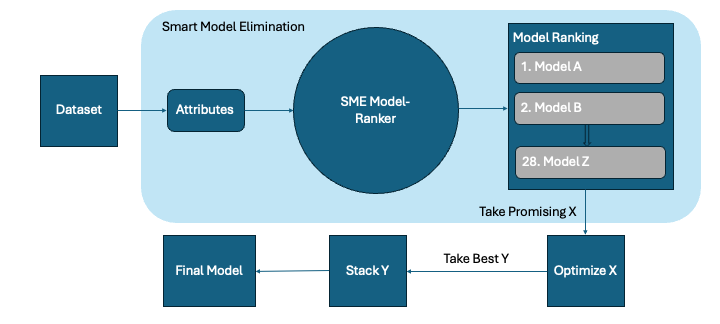
\includegraphics[width=\textwidth]{smeml-flowchart.png}
\caption{Illustration of the SMEML Process}
\end{figure}

\section{Evaluation}
\subsection{Experiment Design}
To evaluate our framework, we choose 5 different datasets of diverse size. We ran SMEML on each dataset for 20 iterations of tuning. We compared this against a "dumb" mode which simply runs every model on the dataset. We used the accuracy and time to train as our metrics. All experiments are run on an Ubuntu server with Intel Xeon E5520 @ 2.27GHz and 24GB of RAM.

\subsection{Experiment Results}
\begin{table}
  \caption{Comparing experiment results for SMEML and dumb mode}
  \label{model-options-table}
  \centering
  \begin{tabular}{llllll}
    \toprule
    % group 2, 3 as multicolumn and 4, 5 as multicolumn
    Dataset & \multicolumn{2}{c}{Accuracy} & \multicolumn{2}{c}{Time to Train (sec)} & Size (RxC)\\
    \cmidrule(lr){2-3} \cmidrule(lr){4-5}
    & SMEML & Dumb & SMEML & Dumb \\
    \midrule
    Lung Cancer Prediction [17] & .9839 & .9839 & 143.07 & 317.04 & 309x16\\
    Chronic Kidney Disease Dataset [18] & 1.0 & 1.0 & 419.64 & 788.46 & 400x26\\
    Pima Indians Diabetes Dataset [19] & .7857 & .8052 & 161.99 & 374.01 & 768x8 \\
    Brain Stroke Prediction Dataset [20] & .9458 & .9458 & 114.16 & 370.95 & 4892x11\\
    Stroke Prediction Dataset [21] & .9393 & .9393 & 172.67 & 385.23 & 5110x12 \\
    Eye State Classification [22] & .9536 & .9549 & 312.57 & 696.51 & 14980x15\\ 
    \bottomrule
  \end{tabular}
\end{table}

The first observation made was that accuracy did not change for 4 of the 6 benchmarks. The other two benchmarks on eye states and diabetes prediction represented a loss of accuracy for SMEML by 0.13\% and 1.95\%, respectively. Training time, however, favored SMEML in every trial. SMEML outperformed the dummy framework by 173.96 seconds in its worst performance on the lung cancer trial and by 383.94 seconds in its best performance on the eye state dataset. Relative to the dummy's performance, a percent decrease in time to run for SMEML of at least 46.78\% could be seen, with a decrease of up to 69.22\% observerd as well. SMEML's worst performance by percent decrease was also the performance in which it returned perfect accuracy. 
\section{Discussion}
\subsection{Summary}
SMEML consistently achieves comparable accuracy to its dumb counterpart while significantly reducing the time required to train the model. Notably, SMEML's performance is not limited by the size of the dataset, achieving its best runtimes--first, third, and fourth fastest overall--on 'large' datasets (those exceeding 1000 rows). SMEML also chose less common algorithms, such as selecting SGDClassifier for the Pima Indians Diabetes Dataset [19] rather than defaulting to industry-standard boosting algorithms [23]. This efficiency and versatility is important in third world medicine where there is a constant influx of new patient data that must be processed quickly. A practical demonstration of this software's real-world application can be found on our SmartDx website [24]. Source code can be found at [25].
\subsection{Limitations}
Our implementation of SMEML has limitations. These include a small training set due to lack of available datasets, finite computing power, time constraints, and a lack of access to paticular scientific literature. Our framework only improves on the model selection process and does not address the various other aspects of AutoML. Therefore, SMEML is not comparable to other full-featured AutoML frameworks.
\subsection{Future Work}
Future work will include increasing the size of the training set, implementing a fully fledged AutoML framework, and conducting a detailed experiment comparing SMEML to other popular AutoML frameworks. 

\begin{ack}
We would like to thank St. Mark's School of Texas for supporting this research.
\end{ack}

\section*{References}

\medskip
{
\small

[1] He, X., et al., “AutoML: A Survey of the State-of-the-Art.” Knowledge-Based Systems 212, 106622 (2021). \url{https://doi.org/10.1016/j.knosys.2020.106622}. 

[2] Nchasi, G., et al., “Challenges Faced by African Healthcare Workers During the Third Wave of the Pandemic.” Health Science Reports 5, 6 (2022). \url{https://doi.org/10.1002/hsr2.893}.

[3] "Global Strategy on Human Resources for Health: Workforce 2030." World Health Organization, pg. 16 (2020). \url{https://www.who.int/publications/i/item/9789241511131}.

[4] Bajwa, J., et al., “Artificial Intelligence in Healthcare: Transforming the Practice of Medicine.” Future Healthcare Journal 8, 188 (2021). \url{https://doi.org/10.7861/fhj.2021-0095}.

[5] LeDell, E., and S. Poirier, “H2O AutoML: Scalable Automatic Machine Learning.” 7th ICML Workshop on Automated Machine Learning (2020). \url{https://automl.org/wp-content/uploads/2020/07/AutoML_2020_paper_61.pdf}.

[6] Olson, S., et al., "Automating Biomedical Data Science Through Tree-based Pipeline Optimization." Applications of Evolutionary Computation 19, 123 (2016). \url{https://doi.org/10.1007/978-3-319-31204-0_9}.

[7] P\l{}o\'{n}ska, A., et al., “MLJAR: State-of-the-art Automated Machine Learning Framework for Tabular Data.  Version 0.10.3.” MLJAR (2021). \url{https://github.com/mljar/mljar-supervised}.

[8] Conrad, F., et al., “Benchmarking AutoML for Regression Tasks on Small Tabular Data in Materials Design.” Scientific Reports 12, 19350 (2022). \url{https://doi.org/10.1038/s41598-022-23327-1}.

[9] Shang, Z., et al., "FLAML: A Fast and Lightweight AutoML Library." 4th MLSys Conference (2021). \url{https://doi.org/10.48550/arXiv.1911.04706}.

[10] Ryzhkov, A., et al., "LightAutoML: AutoML Solution for a Large Financial Services Ecosystem." arXiv:2109.01528 (2021). \url{https://doi.org/10.48550/arXiv.2109.01528}.

[11] Akalin, A., "Computational Genomics With R." Chapman and Hall/CRC, Vol. 1, Section 3.3, (2020). \url{https://compgenomr.github.io/book/relationship-between-variables-linear-models-and-correlation.html}.

[12] Pedregosa, F., et al., "Scikit-learn: Machine Learning in Python." Journal of Machine Learning Research 12, 2825 (2011). \url{https://doi.org/10.48550/arXiv.1201.0490}.

[13] Chen, T., et al., "XGBoost: A Scalable Tree Boosting System." 22nd ACM SIGKDD International Conference on Knowledge Discovery and Data Mining (2016). \url{https://doi.org/10.1145/2939672.2939785}.

[14] Ke, G., et al., "LightGBM: A Highly Efficient Gradient Boosting Decision Tree." Advances in Neural Information Processing Systems 30, 3149 (2017). \url{https://doi.org/10.48550/arXiv.1706.08359}.

[15] Prokhorenkova, L., et al., "CatBoost: Unbiased Boosting with Categorical Features." Advances in Neural Information Processing Systems 32, 6639 (2018). \url{https://doi.org/10.48550/arXiv.1706.09516}.

[16] Head, T. et al., "Scikit-Optimize: Sequential Model-Based Optimization." Zenodo (2020). \url{https://doi.org/10.5281/zenodo.1170575}.

[17] Ms. Nancy Al Aswad, "Lung Cancer" (dataset). \url{https://kaggle.com/datasets/nancyalaswad90/lung-cancer}.

[18] Mansoor Iqbal, "Chronic KIdney Disease Dataset" (dataset). \url{https://kaggle.com/datasets/mansoordaku/ckdisease}.

[19] UCI Machine Learning, "Pima Indians Diabetes Dataset" (dataset). \url{https://www.kaggle.com/datasets/uciml/pima-indians-diabetes-database}.

[20] Izzet Turkalp Akbasli, "Brain stroke prediction dataset" (dataset). \url{https://www.kaggle.com/datasets/zzettrkalpakbal/full-filled-brain-stroke-dataset}.

[21] fedesoriano, "Stroke Prediction Dataset" (dataset). \url{https://kaggle.com/fedesoriano/stroke-prediction-dataset}.

[22] Rob Mulla, "Eye State Classification EEG Dataset" (dataset). \url{https://www.kaggle.com/datasets/robikscube/eye-state-classification-eeg-dataset}.

[23] Mayr, A. et al., "The Evolution of Boosting Algorithms From Machine Learning to Statistical Modelling." Methods Inf Med 2014; 53(06): 419-427. \url{https://doi.org/10.48550/arXiv.1403.1452}. 

[24] SmartDx Website. \url{https://smartdx.vercel.app/}. 

[25] Github Repository. \url{https://github.com/ericspring08/SMEML-Paper}.
}

\end{document}
